\documentclass[a4 paper]{article}
%\usepackage{minted}           %embedding code
\usepackage{amsmath, amsthm, amsfonts} %always use amsmath for symbols, amsthm for theorems 
\usepackage{graphicx}  % for pictures
%\usepackage{lipsum}  % for test text
\usepackage{multicol}    % for multicollumn text
\usepackage[bottom=2.5cm]{geometry}   %to set the margins to your liking
\usepackage[skip = 10pt, indent = 30pt]{parskip}      %to set the distance between paragraphs
\usepackage{tcolorbox}           %for literal color boxes
%\usepackage{witharrows}             % understandable, arrows for equations
\usepackage{tikz}                   %drawings and diagrams
\usetikzlibrary{positioning}        %tikz library for positioning (of nodes?)
\usepackage{pgfplots}               %plotting and graphs
\pgfplotsset{compat=1.18, width = 10cm}
\usepackage{hyperref}
\hypersetup{colorlinks = true, linkcolor = black, urlcolor = blue}
%\usepackage{fancyvrb}           % fancy formatting of verbatim
%\usepackage{fancyhdr, lastpage}
%\pagestyle{fancy} 
%\lhead{Relat\'orio experimento 4}
%\rhead{FisExpI}
%\cfoot{Página \thepage \ de \pageref{LastPage}}
%\usepackage[Bjornstrup]{fncychap} %Sonny, Glenn, Lenny, Conny, Rejne, Bjarne, Bjornstrup
%\usepackage{xcolor}      %color text
\usepackage{siunitx}    %for SI units
\usepackage{setspace}
\onehalfspacing
\usepackage{cleveref}
\usepackage[brazil]{babel}
\usepackage{caption}
\usepackage{subcaption}
\usepackage{pdfpages}
\usepackage{booktabs}
\usepackage{multirow}
\usepackage{textcomp}
\usepackage{amssymb}
\usepackage[document]{ragged2e}
\usepackage{bm}
\usepackage{empheq}




%\setlength{\hoffset}{-2cm}
%\setlength{\voffset}{1.5cm}                     %control your margins however you want!
%\setlength{\marginparwidth}{2cm}
%\setlength{\oddsidemargin}{0cm}

%\newtheorem{theorem}{Theorem}[section]               %how you call it and how you display it
%\newtheorem{corollary}{Corollary}[theorem]


\newcommand{\parag}{\hspace{30pt}}
%\newcommand{\pd}[2]{\frac{\partial#1}{\partial#2}}


\begin{document}
\justifying
\begin{center}{\large Laboratório de Circuitos Elétricos - 02/2024 - Turma 05}\\
{\large \textbf{Experimento 4}}\\ 
28/11/2024
\end{center}

\vspace{500pt}
 \noindent\textbf{Grupo 5:}\\
 Yuri Shumyatsky - 231012826\\
Vinicius de Melo Moraes - 231036274\\
Victor Rizzi Wagner - 231012817


\vspace{30pt}
\newpage

\section{Introdução}

\parag Serão analisados circuitos elétricos de primeira e segunda ordem em experimentos realizados com alimentação por uma fonte de corrente alternada (AC), para que seja possível observar o efeito da mudança de tensão continuamente, em vez de em apenas um instante. Circuitos de primeira ordem, compostos por resistores e capacitores (RC) ou resistores e indutores (RL), apresentam respostas dinâmicas caracterizadas por uma única constante de tempo, enquanto circuitos de segunda ordem, como os RLC, possuem respostas mais complexas, que podem ser oscilatórias ou amortecidas, dependendo de seus parâmetros.

O objetivo do experimento foi investigar o comportamento desses circuitos quando submetidos a uma mudança brusca de tensão, analisando aspectos como amplitude, fase e frequência das grandezas elétricas envolvidas. Através da montagem prática dos circuitos e da medição das tensões e correntes em diferentes componentes, buscou-se validar os modelos teóricos e compreender os fenômenos de ressonância, amortecimento e mudanças de fase.

\vspace{70pt}
\section{Materiais}

	\begin{itemize}
	\item National Instruments Elvis II
	\item 1 capacitor de 47n$C$
	\item 1 indutor de 1m$H$
	\item 1 resistor de 1k$\Omega$
	\item 1 resistor de 47$\Omega$
	\end{itemize}

\newpage
\section{Procedimento}

\parag O National Instruments Elvis é usado como fonte, protoboard, e multímetro. Usa-se a função de multímetro para checar as resistências, capacitância e indutância dos componentes, que são marcadas na Tabela 1.

\vspace{5pt}
\begin{table}[h]
\centering
\begin{tabular}{|c|c|c|c|}
\hline
Grandeza & Valor nominal & Valor medido & Erro (\%) \\\hline
C & 47nF & 46,58nF & \\    \hline
L & 1mH & 0,8694mH & \\    \hline
$R_1$ & 1k$\Omega$ & 0,986k$\Omega$ & \\\hline
$R_2$ & 47$\Omega$ & 46,424$\Omega$ & \\\hline
\end{tabular}
\caption*{Tabela 1: Componentes}
\end{table}

Em seguida, é montado o circuito da Figura 1, usando $R_1=1k\Omega$.

\begin{table}[h]
\centering
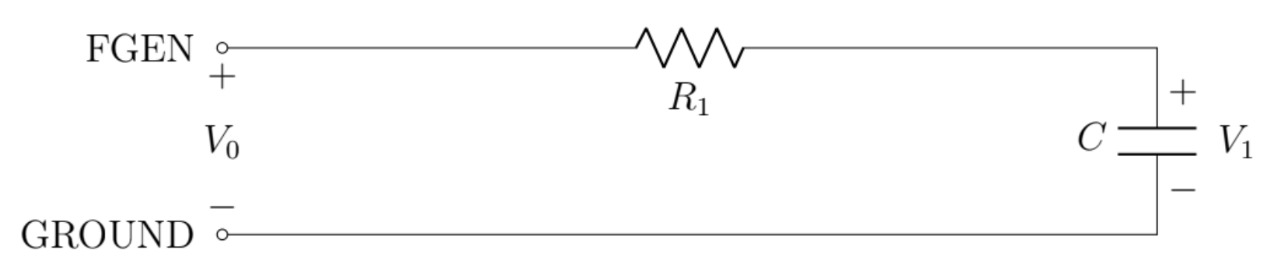
\includegraphics[scale=0.3]{figuras/figura1}
\end{table}

\begin{center}
Figura 1: Circuito de primeira ordem
\end{center}

$\tau$ é calculado usando a fórmula $\tau = R\cdot C$, o que resulta no valor $4,935\cdot10^{-5}s$.

Com isso, podem ser usados os cursores do software do Elvis para fazer a medição em momentos específicos como $t=\tau, t=2\tau, t=3\tau$ e $t=10\tau$ e preencher essas informações na Tabela 2, enquanto a forma da resposta da tensão $V_1$ pode ser vista no Gráfico 1 (A onda quadrada em preto mais escuro é a tensão $V_0$ e a que está em um cinza mais claro é $V_1$).


%cálculos dos nominais


\begin{table}[h]
\centering
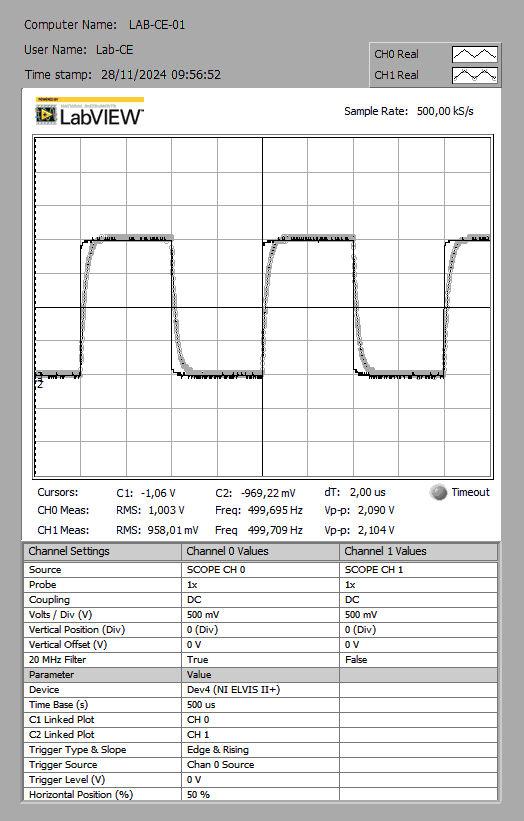
\includegraphics[scale=0.6]{rgadicoas/rgadicoa}
\end{table}

\begin{center}
Gráfico 1: Resposta do circuito RC
\end{center}



\vspace{5pt}
\begin{table}[h]
\centering
\begin{tabular}{|c|c|c|c|}
\hline
Tensão & Valor nominal (V) & Valor medido (V) & Erro (\%) \\\hline
$V_1(0)$ &  & -976,53mV & \\    \hline
$V_1(\tau)$ &  & 281,17mV & \\    \hline
$V_1(2\tau)$ &  & 700,40mV & \\\hline
$V_1(3\tau)$ &  & 910,00mV & \\\hline
$V_1(10\tau)$ &  & 1,04V & \\\hline
\end{tabular}
\caption*{Tabela 2: Tensões para circuito RC}
\end{table}




\newpage
Em seguida, remonta-se o circuito na forma da Figura 2, tornando-se um circuito RLC.

\begin{table}[h]
\centering
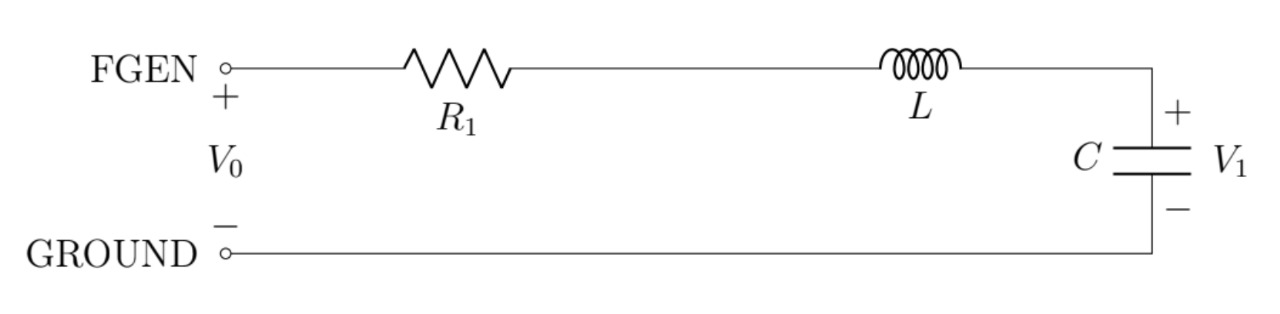
\includegraphics[scale=0.3]{figuras/figura3}
\end{table}

\begin{center}
Figura 2: Circuito de segunda ordem
\end{center}

% cálculos relevantes aqui

Com esses valores e usando o osciloscópio do Elvis, produz-se o Gráfico 2, de onde podem ser medidos os valores que serão preenchidos na Tabela 3. 


\begin{table}[h]
\centering
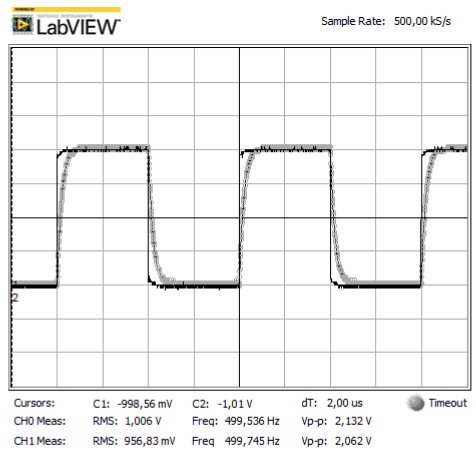
\includegraphics[scale=0.6]{rgadicoas/rgadicoa2}
\end{table}

\begin{center}
Gráfico 2: Resposta do circuito RLC
\end{center}

%mais cálculos relevantes


\vspace{5pt}
\begin{table}[h]
\centering
\begin{tabular}{|c|c|c|c|}
\hline
Tensão & Valor nominal (V) & Valor medido (V) & Erro (\%) \\\hline
$V_1(0)$ &  & -976,53mV & \\    \hline
$V_1(\tau_1)$ &  & 197,32mV & \\    \hline
$V_1(2\tau_1)$ &  & 700,40mV & \\\hline
$V_1(3\tau_1)$ &  & 910,02mV & \\\hline
$V_1(10\tau_1)$ &  & 1,04V & \\\hline
\end{tabular}
\caption*{Tabela 3: Tensões para circuito RLC}
\end{table}


\newpage
Após isso, o resistor $R_1$ é trocado por $R_2=47\Omega$ e todo o procedimento é análogo ao anterior, obtendo os resultados expostos no Gráfico 3 e na Tabela 4.

%cálculos aqui!!!!!
%!!!!!!!!!!!!!!!!!
%!!!!!!!!!!!!!!!!!!!!!
%!!!!!!!!!!!!!!!!!!!!!!!!
%!!!!!!!!!!!!!!!!!!!!!

Porém, é notável uma diferença na resposta, que pode ser vista melhor no Gráfico 4, cuja escala de tempo é ampliada para que a visualização seja mais fácil.


\begin{table}[h]
\centering
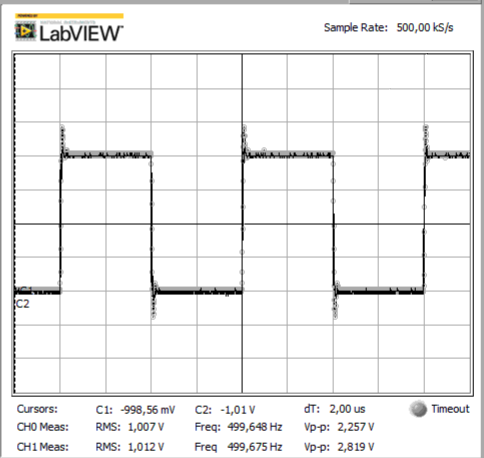
\includegraphics[scale=0.6]{rgadicoas/rgadicoa3}
\end{table}

\begin{center}
Gráfico 3: Resposta do circuito RLC com resistência menor
\end{center}


\vspace{5pt}
\begin{table}[hb]
\centering
\begin{tabular}{|p{5cm}|c|c|c|}
\hline
Grandeza & Valor nominal & Valor medido & Erro (\%) \\\hline
Tempo para $V_1$ atingir seu valor máximo a partir de uma borda de subida da onda quadrada &  & 23,20$\mu$s & \\    \hline
\centering Valor máximo de $V_1$ &  & 1,41V & \\    \hline
\end{tabular}
\caption*{Tabela 4: Circuito RLC com resistência menor}
\end{table}

\newpage
\begin{table}[h]
\centering
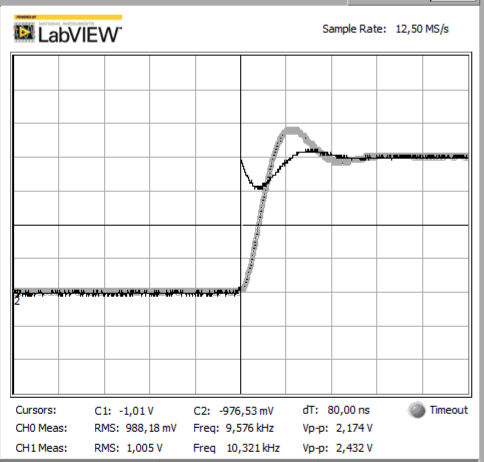
\includegraphics[scale=0.6]{rgadicoas/rgadicoa4}
\end{table}

\begin{center}
Gráfico 4: Resposta do circuito RLC com $R_2$ (ampliado)
\end{center}

A escala de tempo ampliada permite observar com maior clareza os efeitos do amortecimento reduzido sobre a forma da onda. Nota-se um aumento significativo na amplitude das oscilações, indicando uma aproximação ao comportamento subamortecido, devido aos polos serem imaginários.

O tempo necessário para atingir o pico de tensão é menor, enquanto o valor de tensão máxima (1,41 V) foi superior ao do circuito RLC com resistência maior. Esse comportamento é esperado, pois a menor resistência resulta em maior energia disponível para oscilações antes de sua dissipação. 






\newpage
\section{Conclusão}

\parag Os experimentos realizados demonstraram com clareza o comportamento dinâmico de circuitos de primeira e segunda ordem quando submetidos a sinais alternados. No caso do circuito RC, a constante de tempo calculada foi consistente com os dados experimentais, validando a teoria de resposta exponencial para cargas e descargas de capacitores. Para o circuito RLC, foi possível observar fenômenos como ressonância e amortecimento, destacando a influência dos valores de resistência sobre a estabilidade e a frequência da resposta.

A redução da resistência no circuito RLC resultou em uma resposta mais acentuada, evidenciando a diminuição do amortecimento e reforçando a relação entre os parâmetros circuitais e o comportamento oscilatório. 


\vspace{30pt}
\section{Bibliografia}
\begin{itemize}
\item HALLIDAY, D.; RESNICK, R.; WALKER, J. Fundamentos de Física. 10. ed. v. 3. Rio de Janeiro: LTC, 2016.
\end{itemize}


\end{document}